\textbf{1-1} 真空中有两个点电荷 $q_{1}$ 和 $q_{2}$ ，它们的质量分别为 $m_{1}$ 和 $m_{2}$ ，位置矢量分别为 $\pmb{r}_{1}$ 和 $\pmb{r}_{2}$ ，只考虑其间的库仑相互作用。

1. 引入相对位矢 $r = r_2 - r_1$ ，试建立 $r(t)$ 的微分方程。

2. 设 $t = 0$ 时刻, 两点电荷均静止, 相互间距为 $\pmb{r}_0$ . 若两点电荷电量异号, 试问它们何时相碰.
\vfill

\textbf{1-2} 如电图1-2-1，在边长为 $a$ 的正方形的四个顶点分别有电量均为 $Q$ 的固定的点电荷。在正方形对角线交点上放置一个质量为 $m$ 、电量为 $q(q$ 与 $Q$ 同号)的自由点电荷。今将 $q$ 沿某一对角线移动一个很小的距离。试问 $q$ 是否将作周期性振动，若是，试求出振动周期。

\begin{center}
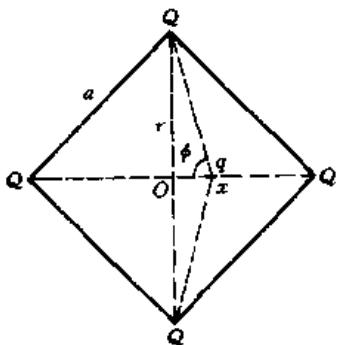
\includegraphics[width=0.2\textwidth]{figures/电图1-2-1.jpg}
\end{center}
\vfill

\newpage
\textbf{1-3} 如电图1-3-1所示，在 $x$ 轴的 $\pm a$ 处分别有两个固定的点电荷，它们的电量均为 $Q(Q > 0)$ 。在 $x$ 轴的 $\pm 2a$ 处分别有另外两个固定的点电荷，它们的电量均为 $-8Q$ 。在原点 $O$ 有一个电量为 $q(q > 0)$ 、质量为 $m$ 的带电质点。设带电质点只能在 $x$ 轴上运动。试分析带电质点所在的平衡位置原点 $O$ ，是否为稳定平衡位置。若原点 $O$ 为稳定平衡位置，将带电质点移到 $x = A$ 处从静止释放 $(0 < A \ll a)$ ，试求其振动周期。
\begin{center}
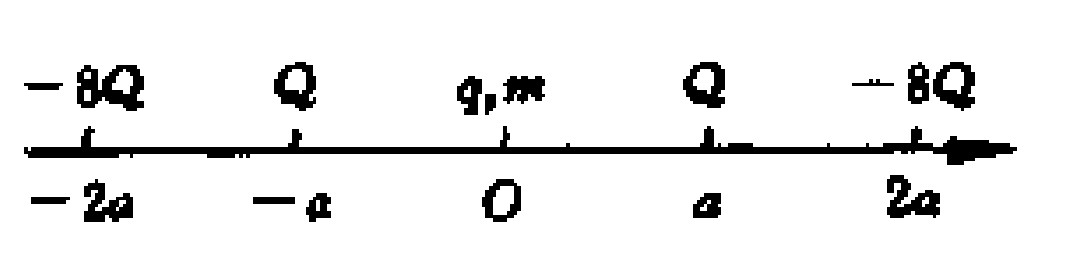
\includegraphics[width=0.2\textwidth]{figures/电图1-3-1.jpg}
\end{center}
\vfill

\textbf{1-4} 电力与距离平方成反比是库仑定律的主要内容。对此，迄今仍有人进行精确的实验检验。试证明，若电力反平方律是精确的，则孤立带电导体球壳达到静电平衡时，其电量将均匀分布在外球面上，球壳内电场强度处处为零。

\vfill

\newpage
\textbf{1-5} 在 $xy$ 平面上有一以坐标原点为圆心，以 $R$ 为半径的带电圆环。电荷线密度的分布为： $y < 0, \lambda = \lambda_0; y > 0, \lambda = -\lambda_0$ 。试求 $z$ 轴（通过圆环的圆心，与圆环所在平面垂直的轴）上的场强分布。
\vfill

\textbf{1-6} 一无限长均匀带电细线弯成如电图1-6-1所示的平面图形，其中AB是半圆弧， $AA'$ 和 $BB'$ 是两平行直线， $A'$ 和 $B'$ 向右端无限延伸．试求圆心O处的电场强度．

\begin{center}
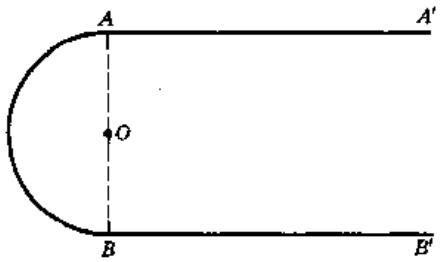
\includegraphics[width=0.25\textwidth]{figures/电图1-6-1.jpg}
\end{center}
\vfill

\newpage
\textbf{1-7} 半径为 $R$ 的半圆环均匀带电，电荷线密度为 $\lambda$ ，试求圆心处的电场强度.
\vfill

\textbf{1-8} 在空间 $A$ 点有电量为 $5Q$ 的固定点电荷，在 $B$ 点有电量为 $12Q$ 的固定点电荷。 $A$ 点和 $B$ 点相距 $13a$ ，空间另一 $C$ 点与 $A$ 点和 $B$ 点分别相距 $5a$ 和 $12a$ 。

1. 以 $C$ 点为球心，以 $r = a$ 为半径作一球。试求在该球区域内，静电场电场强度 $\pmb{E}$ 的平均值

$$
\overline {\boldsymbol {E}} = \frac {\sum_ {i} \boldsymbol {E} _ {i} \Delta V _ {i}}{\sum_ {i} \Delta V _ {i}}
$$

的大小 $|\overline{\boldsymbol{E}}|$ ，式中 $\pmb{E}_i$ 是在体积元 $\Delta V_i$ 处的电场强度。

2. 以 $C$ 点为球心, 以 $r = 10a$ 为半径作一球. 试求在该球区域内, 静电场电场强度 $\pmb{E}$ 的平均值的大小 $|\overline{\pmb{E}}|$ .
\vfill

\newpage
\textbf{1-9} 如电图1-9-1所示，在半径为 $R$ 、体电荷密度为 $\rho$ 的均匀带电球体内部挖去半径为 $R^{\prime}$ 的一个小球, 小球球心 $O'$ 与大球球心 $O$ 相距为 $\alpha$ . 试求 $O'$ 的电场强度, 并证明空腔内电场均匀.

\begin{center}
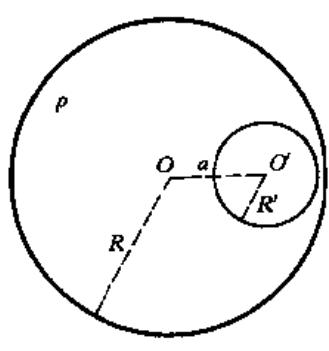
\includegraphics[width=0.2\textwidth]{figures/电图1-9-1.jpg}
\end{center}
\vfill

\textbf{1-10} 如电图1-10-1所示，把半径为 $R$ 的球体切为八等份，取其中一份，使之均匀带电，电荷体密度为 $\rho$ 。试求此八分之一带电球体在球心 $O$ 处的电场强度大小 $E_0$ 。
\begin{center}
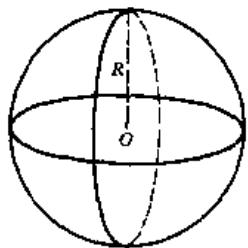
\includegraphics[width=0.2\textwidth]{figures/电图1-10-1.jpg}
\end{center}
\vfill

\newpage
\textbf{1-11} 在惯性系 $S$ 中有匀强电场 $\pmb{E}$ , 其方向如电图1-11-1所示. 在电场中与 $\pmb{E}$ 平行的一条几何直线 (图中画虚线) 上, 有两个静止的小球 A 和 B. 两小球的质量均为 $m$ , A 球所带电量为 $Q(Q > 0)$ , B 球不带电, 开始时两球相距为 $l$ . 在电场的作用下, A 球开始沿直线运动, 并与 B 球发生弹性正碰撞, 从而使 B 球也参与运动. 设在各次碰撞过程中, A 球和 B 球之间并无电量的转移. 设万有引力可略去不计.
\begin{center}
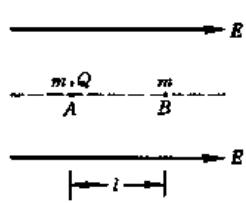
\includegraphics[width=0.2\textwidth]{figures/电图1-11-1.jpg}
\end{center}
试证明，A球与B球相邻两次碰撞之间的时间间隔相同，并求出该时间间隔 $T$
\vfill

\textbf{1-12} 在 $-d \leqslant x \leqslant d$ 的空间区域内，电荷体密度 $\rho > 0$ 为常量。其他区域均为真空。若在 $x = 2d$ 处将质量为 $m$ 、电量为 $q(q < 0)$ 的带电质点自静止释放。试问经多长时间它能到达 $x = 0$ 位置。设带电质点只受电力，其余引力、阻力等均可忽略。
\vfill

\newpage
\textbf{1-13} 在半径为 $R$ 的细圆环上分布着不能移动的正电荷，总电量为 $Q$

1. 如果某个点电荷 $Q_{1} (\neq 0)$ 可在环中指定直径 AOB 线段内作匀速直线运动，试确定圆环上电荷线密度 $\lambda$ 的分布。

2. 取 $x$ 轴沿直径 $AOB$ , 原点 $O$ 在环中心. 将第一问中的点电荷 $Q_{1}$ 放在与 $O$ 点相距 $r_{1}$ 的 $x$ 左半轴上某点. 设电量 $Q_{1}$ 的绝对值为 $Q$ 的 $\nu$ 倍. 能否在 $x$ 右半轴上再放一个非零电量的点电荷 $Q_{2}$ , 使得这两个点电荷及圆环均可保持不动. 设两点电荷都不与环接触, 设环的质量分布均匀. 试求 $Q_{2}$ 及其位置.

3. 把上述两个点电荷 $Q_{1}$ 和 $Q_{2}$ 固定在第二问中确定的位置上, 同时改变它们的电荷符号但保持电量大小不变. 再使环(所带电量 $Q$ 及分布均不变)沿 $x$ 轴的正方向平移一小量 $\delta$ , 然后静止地释放. 试定量讨论环的运动. 设环的质量为 $m$ .

在求解本题时,只需考虑电荷间的库仑作用,其他相互作用均可略.

提示: 把所求的圆环上电荷分布与球面上均匀电荷分布相联系.
\vfill
\newpage

\textbf{1-14} 如电图1-14-1，在半径为 $R$ 、质量为 $m$ 且均匀分布的细圆环上，均匀地分布着总电量为 $q$ 的正电荷。在通过圆环中心 $O$ 点且垂直于圆环平面的 $x$ 轴上有两个固定的点电荷，它们分别在圆环的两侧，与环心的距离均为 $L$ ，各带有电量为 $Q$ 的正电荷.设圆环只能沿 $x$ 轴平动．显然，在上述条件下，圆环处于平衡位置．

\begin{center}
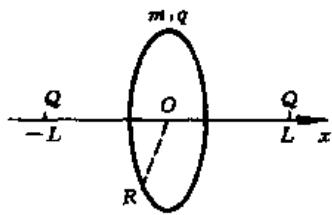
\includegraphics[width=0.25\textwidth]{figures/电图1-14-1.jpg}
\end{center}

1. 试讨论该平衡位置的稳定性(即在什么情况下为稳定平衡位置, 在什么情况下为不稳定平衡位置).

2. 若该位置是稳定平衡位置，试求圆环在其附近作微小振动的周期。
\vfill

\newpage
\textbf{1-15} 如电图 $1 - 15 - 1$ 所示，质量均为 $m$ 、电量均为 $q(q > 0)$ 的一簇带电粒子，从 $P_{1}$ 点以相同速率 $v_{0}$ 在 $xy$ 平面内向右上方各方向射出，即 $\phi$ 角在(0，$\frac{\pi}{2}$ 范围内. 试在 $xy$ 平面内设计一个电场区域, 使这些带电粒子能全部会聚于 $P_{2}$ 点. $P_{1}$ 和 $P_{2}$ 在 $x$ 轴的两侧, 与原点 $O$ 的距离均为 $R$ . 设带电粒子间的相互作用以及引力可略.
\vfill

\textbf{1-16} 如电图1-16-1，两个同心的半球面相对放置，半径分别为 $R_{1}$ 与 $R_{2}(R_{1} > R_{2})$ ，都均匀带电，电荷面密度分别为 $\sigma_{1}$ 与 $\sigma_{2}$ . 试求大的半球底面圆直径AOB上的电势分布.

\begin{center}
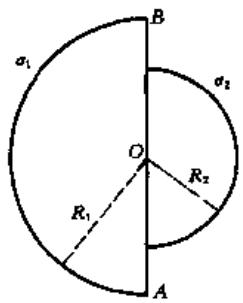
\includegraphics[width=0.15\textwidth]{figures/电图1-16-1.jpg}
\end{center}
\vfill

\newpage
\textbf{1-17} 如电图1-17-1，半径为 $R_{1}$ 的圆环上带有电量 $Q$ ，在它的右边有半径为 $R_{2}$ 的不带电的球面, 球心与环心的间距为 L, 球心与环心的连线和圆环平面垂直. 试求球面上的平均电势 $\overline{U}$ .

\begin{center}
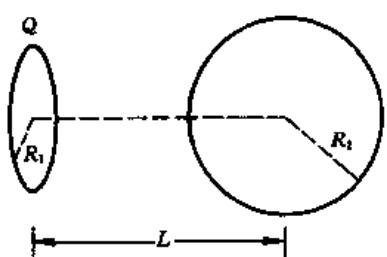
\includegraphics[width=0.25\textwidth]{figures/电图1-17-1.jpg}
\end{center}
\vfill

\textbf{1-18} 地面上有一固定的点电荷A,在A的正上方有一带电小球B,B在重力和A的库仑斥力的作用下,在A上方 $\frac{H}{2}$ 到H之间作往返的自由振动.试求B运动的最大速率 $v_{max}$ .
\vfill

\newpage
\textbf{1-19} 如电图1-19-1所示，两个固定的均匀带电球面A和B分别带电4Q和 $Q(Q>0)$ .两球心之间的距离d远大于两球的半径，两球心的连线MN与两球面的相交处都开有足够小的孔，因小孔而损失的电量可以忽略不计.一带负电的质点静止地放置在A球左侧某处P点，且在MN直线上.设质点从P点释放后刚好能穿越三个小孔，并通过B球球心.试求质点开始时所在的P点与A球球心的距离x应为多少?

\begin{center}
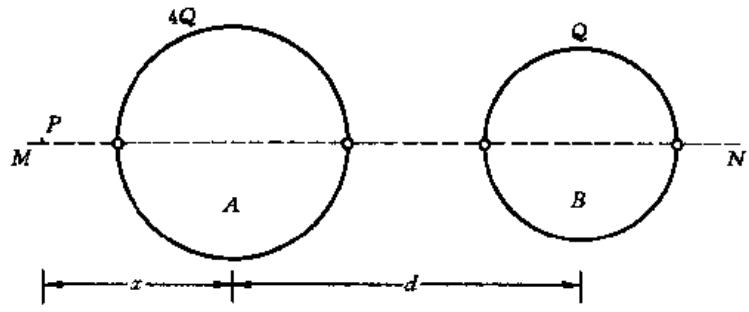
\includegraphics[width=0.3\textwidth]{figures/电图1-19-1.jpg}
\end{center}
\vfill

\textbf{1-20} 半径分别为 $a$ 和 $b$ 的两个同轴无限长半圆柱面如电图1-20-1所示。设在这两个半圆柱面之间有静电场，其电势分布为 $k \ln \frac{b}{r}$ ，其中 $k$ 为某常数， $r$ 是到轴的垂直距离，质量为 $m$ ，电量为 $-q (q > 0)$ 的粒子以初速 $\boldsymbol{v}$ 从图中所示的左方射入， $\boldsymbol{v}$ 既与圆柱面的轴垂直，又与入射处圆柱截面的直径垂直，入射点与轴的距离为 $\rho$ 。

\begin{center}
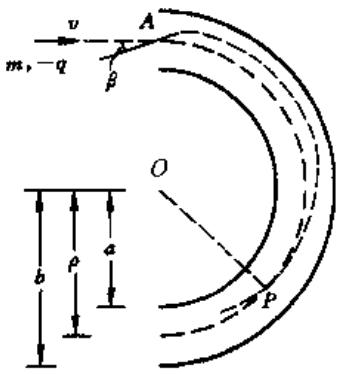
\includegraphics[width=0.15\textwidth]{figures/电图1-20-1.jpg}
\end{center}

1. 试问在什么条件下, 粒子能沿半圆轨道运动.

2. 若入射方向与原设计方向有很小的偏向角 $\beta$ , 如电图1-20-1所示, 那么粒子轨道也将偏离原来的半圆轨道, 设两个轨道的交点为 $P$ . 试证明, 对于很小的偏向角 $\beta, P$ 点的位置与 $\beta$ 无关, 并求出 $P$ 点的方位角 $\angle AOP$ 的大小.
\vfill

\newpage
\textbf{1-21} 在平面上有一段长为 $l$ 的均匀带电直线 $AB$ ，在该平面取直角坐标 $Oxy$ ，原点 $O$ 为 $AB$ 中点， $AB$ 沿 $x$ 轴， $y$ 轴与 $x$ 轴垂直。

1. 试证明, 该平面上任一点 $P$ 的电场强度方向沿 $\angle APB$ 的角平分线.

2. 试求该平面上的电场线方程.

3. 试求该平面上的等势线方程。
\vfill

\textbf{1-22} 如电图1-22-1，在 $x$ 轴的 $-a$ 和 $a$ 两点分别放置电量均为 $Q$ 的点电荷.

试求:1. 在 $xy$ 平面上, 电场强度相对坐标原点 $O$ 为径向的点的轨迹.

2. 在 $xy$ 平面上, 电场强度相对坐标原点 $O$ 为切向的点的轨迹.

(注:所谓径向或切向,均指电场强度 E 的方向相对原点 O 沿径向或切向,并非 E 的径向或切向分量.)

\begin{center}
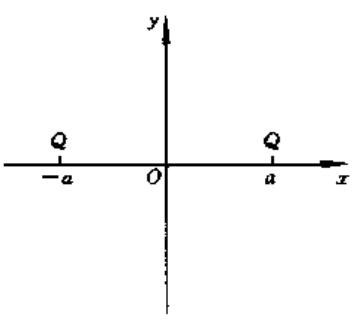
\includegraphics[width=0.25\textwidth]{figures/电图1-22-1.jpg}
\end{center}
\vfill

\newpage
\textbf{1-23} 线电荷密度分别为 $\lambda$ 和 $-\lambda (\lambda =$ 常量）的两平行无限长带电直线相距 $2a$ ，试求等势面和电场线的空间分布．
\vfill

\textbf{1-24} 已知真空中电场的能量密度为 $w_{\mathrm{e}} = \frac{1}{2}\varepsilon_0E^2$ . 试求:

1. 均匀带电球面 (电量为 $Q$ , 半径为 $R$ ) 的球面上的电场强度值. 

2. 带电球面上的表面张力系数 $\sigma$ .
\vfill

\newpage
\textbf{1-25} 有1998个半径相同的导体球，各球均带有相同的正电荷，彼此不接触。试证明，在静电平衡时，至少有一个导体球的表面处处无负电荷。
\vfill

\textbf{1-26} 质子加速器使每个质子得到的动能为 $E$ 。很细的质子束从加速器射向一个远离加速器的半径为 $r$ 的金属球，并留在球上。球的中心并不处在加速器发射出的质子运动方向的直线上，而与该直线的垂直距离为 $d$ ，且 $d < r$ 。试问加速器工作足够长时间后，球能充电到多高的电势？

计算时, 可取 $E = 2 \text{kev}$ 和 $d = \frac{r}{2}$ . 又, 若把质子换成电子, 将会发生什么变化?
\vfill

\newpage
\textbf{1-27} 如电图1-27-1所示，导体球A、B和C的半径分别为 $2\mathrm{cm}, 2\mathrm{cm}$ 和 $3\mathrm{cm}$ ，它们的球心构成边长为 50 cm 的等边三角形 ABC. 开始时, A、B、C 三球各带电荷 $12 \times 10^{-9}$ C、 $24 \times 10^{-9}$ C、 $30 \times 10^{-9}$ C, 试求 B 球电势的近似值, 并估算所用近似方法产生的误差.

若将三球用导线彼此相连,忽略连接后导线上的电荷分布,试求各球所带电量.

设 Ox 轴通过 $\triangle ABC$ 的中心，并垂直于 $\triangle ABC$ 所在平面。试计算导线将三球连接后，在 Ox 轴上与 O 点的距离等于 CO 的那一点的电场强度。

\begin{center}
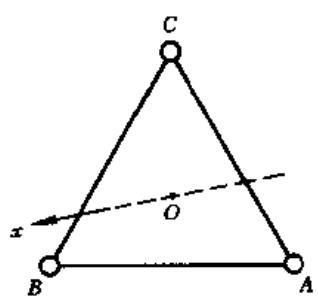
\includegraphics[width=0.15\textwidth]{figures/电图1-27-1.jpg}
\end{center}
\vfill

\textbf{1-28} 如电图1-28-1所示，在真空中有四个半径均为 $a$ 的不带电的相同导体球，球心分别位于边长为 $r$ 的正方形的四个顶点之上， $r \gg a$ 。现让球1带 $Q$ 的电荷 $(Q > 0)$ ，然后取一细金属丝, 它的一端固定在球 1 上, 另一端分别依次与球 2、3、4 接触. 设每次接触的时间都足够长, 使它们达到静电平衡后, 再断开. 设分布在细金属丝上的电荷可忽略不计. 试求四小球最后所带电量 $Q_{1}, Q_{2}, Q_{3}, Q_{4}$ .

\begin{center}
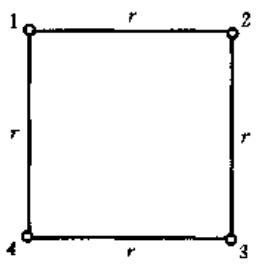
\includegraphics[width=0.15\textwidth]{figures/电图1-28-1.jpg}
\end{center}
\vfill

\newpage
\textbf{1-29} 如电图1-29-1所示,三根等长的带电绝缘细棒首尾相接构成三角形,其中电荷的分布如同绝缘棒都换成等长导体棒且已达到静电平衡时的电荷分布。测得图中 $A$ 点和 $B$ 点的电势分别为 $U_{A}$ 和 $U_{B}$ 。假设若将 $ab$ 棒取走，并不影响 $ac$ 及 $bc$ 两棒的电荷分布。试求此时 $A$ 点和 $B$ 点的电势。

\begin{center}
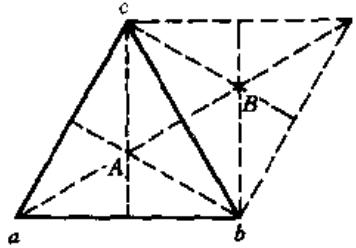
\includegraphics[width=0.2\textwidth]{figures/电图1-29-1.jpg}
\end{center}
\vfill

\textbf{1-30} 如电图 $1 - 30 - 1$ 所示，恒温的矩形盒内装有理想气体，当隔板将盒等分为二时，两侧气体压强均为 $P_{0}$ 。当隔板平行移动时，无摩擦，不漏气，两侧气体经历准静态过程。隔板是面积为 $A$ 的金属板，带电量为 $Q$ ，矩形盒上与它平行的两块板也是金属板，面积也为 $A$ ，相距为 $2L$ ，固定，并接地。隔板两侧的电场均匀。盒的其余部分是不导电的绝缘板。

1. 试求隔板的平衡位置。

2. 试讨论平衡是否稳定。
\begin{center}
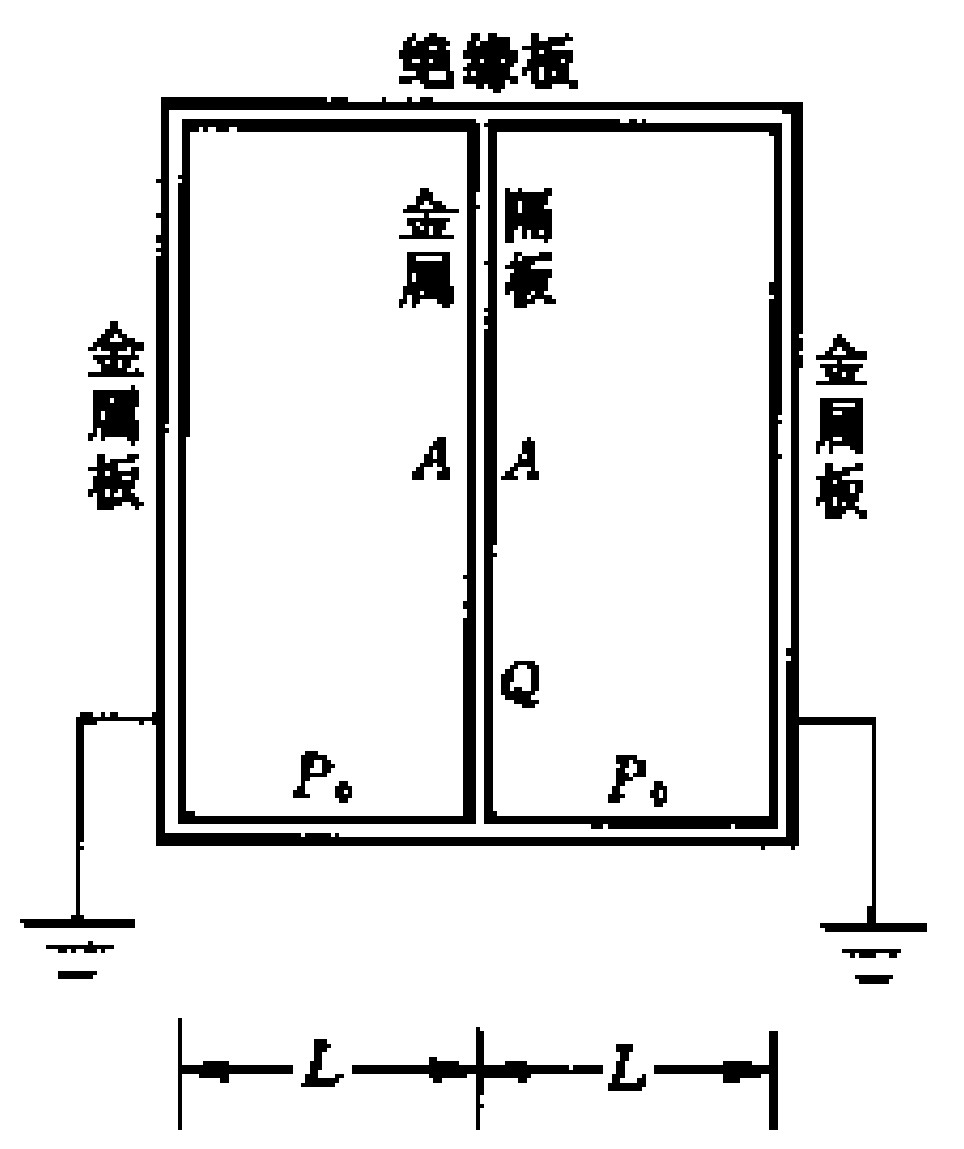
\includegraphics[width=0.1\textwidth]{figures/电图1-30-1.jpg}
\end{center}
\vfill

\newpage
\textbf{1-31} 如电图1-31-1所示，在半径为 $R$ 的接地金属圆柱面的中央放有一根半径为 $r_0$ 的同轴细长导线，导线处于正的高电势 $U_0$ 。于是导线外侧附近介质原子被电离成自由电子与正离子，其中自由电子即被导线吸附,正离子则离开导线径向地运动.设正离子的径向迁移率(径向速度与电场强度的比值)为常数w,且迁移过程中正离子始终围绕导线形成均匀的圆柱形薄层.

\begin{center}
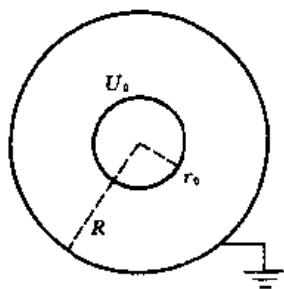
\includegraphics[width=0.3\textwidth]{figures/电图1-31-1.jpg}
\end{center}

1. 试证明,作为时间 $t$ (从正离子在导线外侧附近形成的时刻开始计时)的函数,正离子的径向位置 $\boldsymbol{r}$ 可表为
$$
r ^ {2} = k (t + t _ {0})
$$
并求出常量 k 和 $t_{0}$ (略去由于介质电离造成的电场变化).

2. 设全部正离子电量为 Q，为了使导线电势保持原来的 $U_{0}$ 不变，需给导线补充电量 $Q^{*}$ . 试导出 $Q^{*}$ 与时间 t 的关系.
\vfill

\textbf{1-32} 圆形导体薄板的半径为 $R$ ，在其中轴线上与圆板中心 $O$ 相距为 $a$ 处有一个静止的点电荷 $Q$ .设 $a\ll R$ ，忽略边缘效应.

1. 导体板接地，试求导体板上的电荷分布。

2. 导体板不接地, 带有电量 $Q_{0}$ , 试求导体板上的电荷分布.
\vfill

\newpage
\textbf{1-33} 如电图1-33-1所示，两块足够大的接地导体平面A和B平行竖直放置，相距 $2d$ ， $d = 10\mathrm{cm}$ .在两板之间的中央位置，用长 $l = 1\mathrm{m}$ 的绝缘细线悬挂一个质量 $m = 0.1\mathrm{g}$ ，电量 $q = 5\times 10^{-9}\mathrm{C}$ 的小摆球．让小摆球稍稍偏离平衡位置后释放，使之小角度摆动．忽略各种电磁阻尼和空气阻尼．试求小球的摆动周期 $T$

\begin{center}
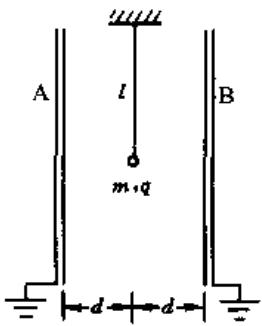
\includegraphics[width=0.2\textwidth]{figures/电图1-33-1.jpg}
\end{center}
\vfill

\textbf{1-34} 半径为 $R$ 的导体球带有电量 $Q(Q > 0)$ 。今在距球心为 $a$ 处 $(a > R)$ 放置一个与 $Q$ 同号的点电荷 $q$ 。为使导体球在静电平衡时受到 $q$ 的作用力吸引，试确定 $q$ 的取值范围。
\vfill

\newpage
\textbf{1-35} 两个半径均为 $R$ 的导体球相互接触形成一孤立导体，试求此孤立导体的电容。
\vfill

\textbf{1-36} 在空间 $n$ 个点上依次放置 $n$ 个点电荷 $q_{1}, q_{2}, \cdots, q_{n}$ , 这些电荷在这 $n$ 个点上产生的总电势分别记为 $U_{1}, U_{2}, \cdots, U_{n}$ . 若在这 $n$ 个点上换成另一组点电荷 $q_{1}^{\prime}, q_{2}^{\prime}, \cdots, q_{n}^{\prime}$ , 则相应的总电势为 $U_{1}^{\prime}, U_{2}^{\prime}, \cdots, U_{n}^{\prime}$ . 试证明
$$
\sum_ {i = 1} ^ {n} q _ {i} U _ {i} ^ {\prime} = \sum_ {i = 1} ^ {n} q _ {i} ^ {\prime} U _ {i}, \quad n \geqslant 2
$$
由此进一步证明, 真空中由一对导体构成的电容器的电容与这两个导体的带电量多少无关.
\vfill

\newpage
\textbf{1-37} 如电图1-37-1所示，A和B是两块相同的水平平行金属板，相距为 $d$ ，构成电容为 $C$ 的平行板电容器.B板接地，B板中有一个小孔，开始时A和B均不带电.在B板小孔上方 $h$ 处，不断有带电小液珠从静止开始自由下落(空气阻力可略)，每个液珠的电量为 $q$ ，质量为 $m$ ，液珠经小孔到达A板后被吸收，液珠的下落保持一定的间隙，即在前一液珠被A板吸收并达到静电平衡后，后一液珠才继续下落．试问有多少个液珠能落到A板上.

\begin{center}
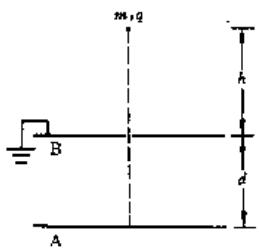
\includegraphics[width=0.2\textwidth]{figures/电图1-37-1.jpg}
\end{center}
\vfill

\textbf{1-38} 如电图1-38-1所示,两个相同的水平放置的平板空气电容器连接起来,充电后电容器A中的带电微粒P刚好静止地悬浮着.撤去电源,将电容器B的两板水平地错开,使两板相对的面积减小为原来的一半.试求此时带电微粒P在竖直方向运动的加速度.

\begin{center}
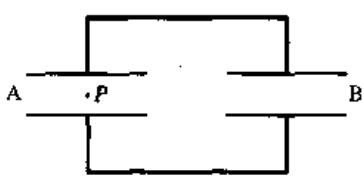
\includegraphics[width=0.2\textwidth]{figures/电图1-38-1.jpg}
\end{center}
\vfill

\newpage
\textbf{1-39} 如电图1-39-1所示，一个边长为 $L$ 的正方形平板电容器，板面竖直地串联在线路中.线路中的直流电源确保电压稳定，为 $V_{0},\mathbf{G}$ 是电流计．一块矩形金属板，垂直于图面方向的长度也为 $L$ ，高为 $L^{\prime}(L^{\prime}\ll L)$ ，厚为 $\frac{D}{P} (D$ 是电容器两板的间距， $P\gg 1$ 是一个系数).开始时，金属板竖直地放在电容器中线(在电图1-39-1中用虚线表示)的正上方，其下端与电容器两板的上端对齐，然后自由落下．忽略各种边缘效应，忽略电磁力对金属板的作用．

试求电容器极板上的电量 Q 随时间 t 的变化关系，并画出流过电流计的电流 I 随时间 t 的变化图线（如电图 1-39-1，设从上到下流过电流计的电流为正，反之为负）.

\begin{center}
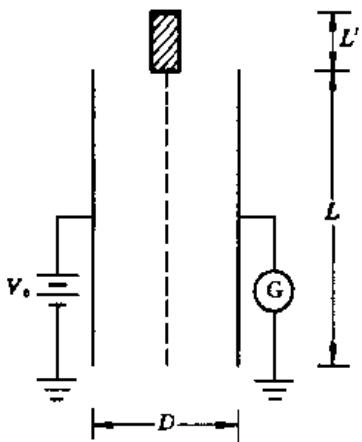
\includegraphics[width=0.15\textwidth]{figures/电图1-39-1.jpg}
\end{center}
\vfill
\newpage

\textbf{1-40} 由直流电源、电容、电阻和开关 K 构成的网络如电图1-40-1所示，其中电源的电动势为 E，三个电容器 $C_{1}$ 、 $C_{2}$ 、 $C_{3}$ 的电容均为 C，两个电阻器的电阻分别为 $R_{1}$ 和 $R_{2}$ 。开始时，三个电容器均不带电，先接通 Oa，再接通 Ob，再换接 Oa，再换接 Ob，…，如此反复换向。设每次换接前都已达到静电平衡。
\begin{center}
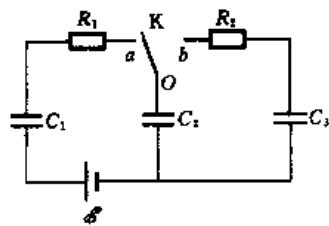
\includegraphics[width=0.25\textwidth]{figures/电图1-40-1.jpg}
\end{center}
试求:1. 第 n 次接通 Ob 并达到静电平衡后, 各电容器两端的电压分别是多少? 2. 当反复换向无穷多次后, 在所有电阻上消耗的总电能是多少?
\vfill

\newpage
\textbf{1-41} 两块长与宽均为 $a$ 与 $b$ 的导体平板在制成平行板电容器时稍有偏斜，使两板一对宽边相距为 $d$ ，另一对宽边相距为 $(d + h)$ ，且 $h \ll d$ 。若此电容器内充满了相对电容率为 $\varepsilon_r$ 的电介质。试求电容器的电容。
\vfill

\textbf{1-42} 如电图1-42-1，两个同轴导体圆筒，内筒半径为 $R$ ，两筒间距为 $d$ ，简高为 $L$ ，且 $L \gg R \gg d$ 。内筒外筒与电源的负极连接．圆筒的中央轴在铅垂线上，筒间 A 和 B 两点的连线与中央轴平行，A 点和 B 点的间距为 h．一个质量为 m，电量为 $-Q(Q>0)$ 的带电粒子从 A 点射出，其速率为 $v_{0}$ ，速度的方向垂直于由 A 点和筒中央轴线确定的平面．为了使该带电粒子能经过 B 点，试求所有可供选择的 $v_{0}$ 和 $C_{x}$ 值．

\begin{center}
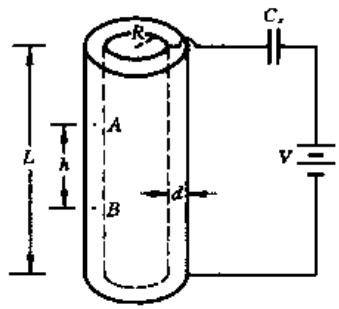
\includegraphics[width=0.2\textwidth]{figures/电图1-42-1.jpg}
\end{center}
\vfill

\newpage
\textbf{1-43} 如电图1-43-1所示，金属球壳上方与一个带有两个活栓的细长玻璃管连接，管壁外包着金属箔，金属箔与电池组的接地端连通，管上方槽中的水银则与电池组另一端正极连通，开始时，球内无水银且不带电，玻璃管下端的活栓关闭，上端的活栓打开，管内充满水银，然后，关闭上端活栓，移开金属箔，再打开下端活栓，使管内水银注入球内。不断重复此过程，直至球内充满水银为止。设电池组的端电压为 $V$ ，玻璃的相对电容率（又称介电常量）为 $\varepsilon_r$ ，管半径为 $r$ ，管壁厚度为 $d$ ，球半径为 $R$ ，且有 $R \gg r \gg d$ 。试近似计算金属球壳充满水银后相对于地的电势。
\begin{center}
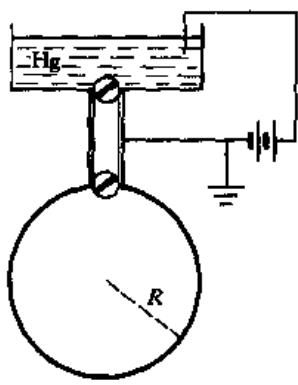
\includegraphics[width=0.2\textwidth]{figures/电图1-43-1.jpg}
\end{center}
\vfill
